\chapter{Caso de Teste}

\section{Apresentação do Sistema}

Para ilustrar o funcionamento do sistema supervisório, foi utilizado um Arduino UNO que simulasse o funcionamento de um processo com dois tanques de área variável acoplados. A Figura abaixo o esquematiza:

\begin{figure}[H]
	\centering
	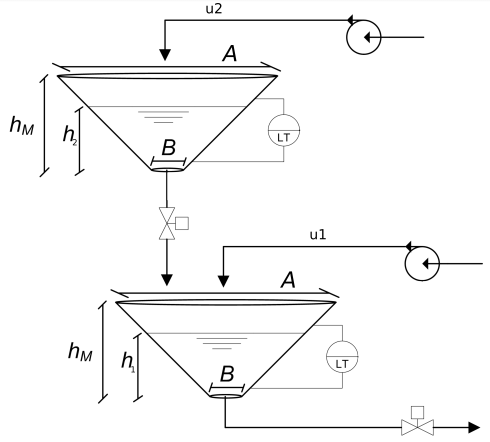
\includegraphics[width=0.8\textwidth,height=0.4\textheight]{sistema_teste}
	\caption{Esquema de leitura serial no supervisório didático\\Fonte: Elaborado pelo Prof. Daniel Santana}
	\label{img_sistema_teste}
\end{figure}

Como percebido pelo esquema, os tanques têm o formato de tronco de cone e a variável controlada é a sua altura. O controle é feito por 2 bombas que aumentam ou diminuem a vazão de entrada de fluido em ambos os tanques. A medição é realizada por dois sensores de nível, sujeito a ruídos brancos.

As equações deste processo são descritas abaixo:
\\\\
$
\frac{dh_1}{dt} = \frac{1}{\beta(h_1)}(u_1 - k\sqrt{\rho g h_1} + k\sqrt{\rho g h_2})\\
\frac{dh_2}{dt} = \frac{1}{\beta(h_2)}(u_2 - k\sqrt{\rho g h_2})\\
\beta(h_i) = frac{dV}{dh_i}\\
V(h_i) = \frac{\pi\gamma^2}{3}(h_i + \frac{B}{2\gamma})^3 - \frac{\pi}{3\gamma}(\frac{B}{2})^3\\
\gamma = \frac{A-B}{2h_M}\\
$

Seus parâmetros e variáveis são descritos e dimensionados na tabela \ref{tbl_parameters}:

\begin{table}[H]
	\centering
	\begin{tabular} {|m{5em}|m{15em}|m{8em}|}
		\hline
		Símbolo & Descrição & Valor (u.m.) \\
		\hline
		A & diâmetro superior & 4 ($m$) \\
		B & diâmetro inferior & 1 ($m$) \\
		hm & altura máxima & 4 ($m$) \\
		V & volume & - ($m^3$) \\
		h & altura & - (m) \\
		$\rho$ & densidade do fluido & 1000 ($kg/m^3$) \\
		g & aceleração da gravidade & 9,8 ($m/s^2$) \\
		k & constante de descarga no tanque & 0,001 (-)\\
		u & vazão da bomba & - ($m^3/s$)\\
		\hline
	\end{tabular}
	\caption{Tabela de parâmetros e variáveis do sistema}
	\label{tbl_parameters}
\end{table}

\section{Sintonia do Controlador}

Por tratar-se de um sistema não linear, serão comparados dois controladores sintonizados por métodos distintos. No primeiro caso, o sistema será linearizado em torno de um ponto de operação e o resultado será utilizado para sintonizar um controlador PID. Em seguida o controlador será acoplado ao sistema. No segundo caso, será utilizada uma lei de controle que anula a não-linearidade do sistema, transformando-o em uma sistema linear. Após este passo, também será utilizado um controlador PID para controlá-lo.

\subsection{Linearização do Sistema}

O processo de linearização de um sistema consiste na aplicação da série de Taylor em suas equações descritivas num determinado ponto de operação.

\begin{figure}[H]
	\centering
	$
	f(x1, x2, .. , xn) \simeq f(x1_0, x2_0, ..., x3_0) + \bigg( \sum_{i=1}^n \frac{df}{dxi}\big|_{xi=xi_0} (xi - xi_0) \bigg)
	$
	\caption{Série de Taylor truncada na primeira ordem}
\end{figure}

sendo a expressão $(xi - xi_0)$ chamada de desvio e representada por $\overline{xi}$.

Aplicando a linearização no sistema de estudo, as novas equações do sistema, em desvio, serão então:
\\\\
$
\frac{dh_1}{dt} = -\big(\frac{d\beta^{-1}(h)}{dh}\bigg|_{{h_1}_{ss}} k\sqrt{\rho g {h_1}_{ss}} + \frac{\beta^-1({h_1}_{ss}) k\sqrt{\rho g}}{2\sqrt{{h_1}_{ss}}}\big)\overline{h_1} + \big(\frac{\beta^-1({h_1}_{ss}) k\sqrt{\rho g}}{2\sqrt{{h_2}_{ss}}}\big)\overline{h_2} +  \beta^{-1}({h_1}_{ss})\overline{u_1}
$
\\
$
\frac{dh_2}{dt} = -\big(\frac{d\beta^{-1}(h)}{dh}\bigg|_{{h_2}_{ss}} k\sqrt{\rho g {h_2}_{ss}} + \frac{\beta^-1({h_2}_{ss}) k\sqrt{\rho g}}{2\sqrt{{h_2}_{ss}}}\big)\overline{h_2} + \beta^{-1}({h_1}_{ss})\overline{u_2}
$
\\
$
\beta^{-1}(h) = \frac{4}{4\pi(\gamma h)^2 + 4B\gamma h + B^2} 
$
\\
$
\frac{d\beta^{-1}(h)}{dh} = -4 \frac{8 \pi \gamma^2 h + 4 \gamma B}{(4\pi(\gamma h)^2 + 4B\gamma h + B^2)^2}
$

De forma a zerar a função $\frac{dh_i}{dt}$ presente na série de Taylor, define-se como um bom ponto de operação um dos estados estacionários do sistema, como por exemplo,  $h_{1_0}=h_{1_{ss}}=1, h_{2_0}=h_{2_{ss}}=1, u_{1_0}=u_{1_{ss}}=0, u_{2_0}=u_{2_{ss}}=k\sqrt{\rho g}$. Substituídos os parâmetros de acordo com a tabela \ref{tbl_parameters} e em formato de espaço de estados o sistema final linearizado será
\\\\
$
\begin{pmatrix} \dot{\overline{h_1}} \\ \dot{\overline{h_2}} \end{pmatrix} = \begin{pmatrix} -0,063 & 0,046 \\ -0,063 & 0 \end{pmatrix} \begin{pmatrix} \overline{h_1} \\ \overline{h_2} \end{pmatrix} + \begin{pmatrix} 0,937 & 0 \\ 0 & 0,937 \end{pmatrix} \begin{pmatrix} \overline{u_1} \\ \overline{u_2} \end{pmatrix}
$
\\\\
\subsection{Sintonia do LQI}

\subsection{Sintonia do PI}

O controlador PI é um tipo bastante utilizado na indústria. Possui um ganho proporcional (P) e um ganho integrativo (I), que incidem sobre a diferença entre a medição atual de uma saída de processo e seu valor desejado. Isto exige que o sistema de controle seja realimentado com um valor geralmente advindo de um sensor, constituindo-o num sistema de malha fechada. A sintonia de um PI se traduz na definição de P e I, e pode ser realizada, entre outras formas, por métodos como Ziegler-Nichols, Coher-Coon ou até mesmo tentativa e erro.

Sendo $P(s)$ uma função de transferênciaentre a saída $Y$ de um processo e sua única entrada $u$, um método simples de sintonia, que dispensa experimentação é o chamado síntese direta.
Tomando um sistema em malha fechada representado na figura \ref{img_exemplo_processo}

\begin{figure}[H]
	\centering
	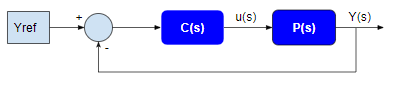
\includegraphics[width=0.8\textwidth]{exemplo_processo}
	\caption{Processo 1x1 com feedback e controlador}
	\label{img_exemplo_processo}
\end{figure}

sua função de tranferência entre a saída $Y$ e entrada $u$ será
\\\\
$
\frac{Y(s)}{u(s)} = \frac{C(s)P(s)}{1+P(s)C(s)}
$
\\

Desta forma, caso deseje-se modelar $Y(s)$ como uma função de primeiro grau $\frac{1}{\tau s + 1}$, a equação do controlador $C(s)$ assumirá
\\\\
$
C(s) = \frac{P^{-1}(s)}{\tau s}
$
\\

Caso $P$ seja uma função de primeiro grau, o controlador será um PI.

Para este método de sintonia, o cálculo dos ganhos do controlador de $h_1$ desconsidera a influência de $h_2$. Tomando como base o sistema linearizado e aplicando a equação da malha fechada, o mesmo será
\\\\
$
\overline{h_1}(s) = \frac{0,937}{s + 0,063} \overline{u_1}(s) + \frac{0,046}{s + 0,063} \overline{h_2}(s) 
$
\\
$
\overline{h_2}(s) = \frac{0,937}{s + 0,063} \overline{u_2}(s)
$
\\\\
logo, os controladores, projetados para um tempo de resposta $\tau$ de 10 segundos, serão:
\\\\
$
C_1(s) = C_2(s) = \frac{1}{10s} \frac{s + 0,063}{0,937} = 0,1067 + 0,0067 \frac{1}{s}
$
\\

\section{Configuração do supervisório didático}

Como já mencionado, o programa apresentado implementa duas funções que podem ser editadas pelo usuário, de forma que seja possível uma resposta ao dispositivo conectado. O usuário pode ainda escrever suas próprias funções e alterar os objetos do código fonte como preferir, para atender as suas necessidades. 

\subsection{LQI}

\subsection{Controlador PI}

Além da biblioteca \emph{python-control}, existe outra chamada emph{simple-pid} que, como o nome indica possui objetos que se comportam como controladores PID. Eles recebem como parâmetrosseus respectivos ganhos, valor de referência da variável controlada, limites para a resposta e outros que são referenciados  \href{https://pypi.org/project/simple-pid/}{na página da biblioteca}. Para implementá-los no programa, na função \emph{setup\_control()}, criam-se tais objetos de acordo com o código abaixo:
\\\\
\texttt{\footnotesize self.pids = [] \\
	self.pids.append(simple\_pid.PID(0.1067, 0.0067, setpoint=1, output\_limits=(None, None))) \\
	self.pids.append(simple\_pid.PID(0.1067, 0.0067, setpoint=1, output\_limits=(None, None)))}
\\\\
O objeto PID, quando chamado, retorna um valor numérico referente à resposta do controlador a partir de uma leitura, informada como parâmetro. Este valor pode ser escrito na porta serial, e será capturado pelo dispositivo conectado, desde que o mesmo esteja preparado para recebê-lo. No Arduino, o comando \emph{\textbf{Serial}.parseFloat()} se mostrou satisfatório.

Implementando na função \emph{loop\_control()} a lógica descrita acima:
\\\\
\texttt{\footnotesize def loop\_control(self, last\_row\_read): \\
	\hspace*{8mm}if len(last\_read) == 0: \\
	\hspace*{8mm}\hspace*{8mm} return \\\\
	\hspace*{8mm}signals = [self.pids[i](input\_value) for i, input\_value in enumerate(last\_row\_read)] \\
	\hspace*{8mm}for signal in signals: \\
	\hspace*{8mm}\hspace*{8mm}self.porta.write('{:.2f}'.format(signal).encode('UTF-8')) \\
	\hspace*{8mm}return}
\\\\
